\subsection{Accelerometer}
Et accelerometer er et elektromekanisk apparat, som anvendes til at måle accelerationskræfter, hvilket er ændringer i hastighed og position \citep{Goodrich2013,TittertonWeston2004}. Enheden for dette er $m/s^2$ eller g-kræfter, idet 1 g svarer til 9,82$m/s^2$. Et accelerometer måler dermed egenaccelerationen af et givent objekt. \fxnote{En g-kraft på jorden svarer til tyngdekraften på 9,82$m/s^2$, men varierer med elevation. Wiki har en god forklaring af dette, hvis man stadig er i tvivl.}\citep{Sparkfun,TittertonWeston2004} \newline

Et accelerometer måler to former for acceleration, henholdsvis statisk og dynamisk. De statiske kræfter er tyngdekraften og vinkelretning af accelerometeret. De dynamiske kræfter beskriver retningen af accelerometerets bevægelse og dets vibrationer. \citep{Sparkfun,Engineering, Goodrich2013}. Der findes accelerometre, som har en, to eller tre måleakser. For at opnå det fulde udbytte af et accelerometer bør et tre-akse accelerometer benyttes eller tre single-akse accelerometre, som placeres vinkelret på hinanden. \citep{TittertonWeston2004} 

Accelerationen i et accelerometer beregnes ud fra Newtons anden lov, $F=ma=mf+mg$, hvor den totale kraft (F), er lig med den påvirkede masse (m), ganget med dets acceleration (a). Dette kan også defineres som summen de eksterne kræfter (f) ganget med massen (m) og tyngdekræften (g) ganget med massen (m). \citep{TittertonWeston2004,Academic2016d} \newline
Illustrativt kan et accelerometer beskrives som en kapsel, hvori der er en indre masse spændt mellem to fjedre, hvilket illustreres på \figref{acc_simpelt}. Ændringen af den indre masse i den sensitive akse kan dermed beskrive accelerationen af selve accelerometeret i den pågældende akse. Hvis accelerometeret kastes op i luften, vil både kapslen og den indre masse udelukkende påvirkes af tyngdekræften, og der vil derfor ikke registeres en acceleration.\citep{TittertonWeston2004,Academic2016d} \newline

\begin{figure}[H]
	\centering
	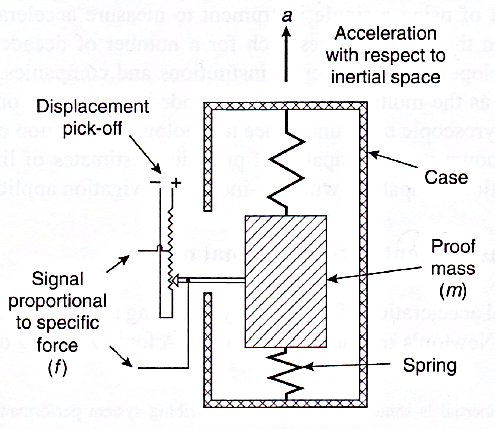
\includegraphics[scale=0.5]{figures/bProblemloesning/accelerometer_basic.png}
	\caption{På figuren fremgår opbygningen af et accelerometer med en indre masse, fjedre og den ydre kapsel. \citep{TittertonWeston2004} (Modificeret)}
	\label{acc_simpelt}
\end{figure}
Ethvert stillestående objekt påvirkes af 1 g i den vertikale akse \citep{Serway2010}. Derfor vil et stillestående accelerometer altid påvirkes af $\pm$1g på én bestemt akse afhængig af sensorens orientering. Eksempelvis, hvis accelerometeret er placeret på et bord med dets positive y-akse i vertikal retning, da vil y-aksen blive påvirket med $+$1 g. I dette tilfælde vil de andre akser, henholdsvis x-, og z-aksen, ikke blive påvirket af nogen kræfter, med antagelse om idelle betingelser. 

Accelerometre benyttes enten i en åben eller lukket kreds. I en åben kreds fastholdes den indre masse til et nulpunkt ved at være udspændt mellem to fjedre. Ved acceleration af den ydre kapsel bevæges den indre masse væk fra nulpunktet, hvorved ændringen for et single-akse accelerometer vil være proportional med kræften, som påvirker systemet. \newline
I en lukket kreds fastholdes den indre masse til et nulpunkt ved hjælp af magnetiske kræfter. Oftest påmonteres en spole på den indre masse, hvormed magnetfeltet forstærkes. Det er muligt at foretage mere præcise målinger omkring nulpunktet end ved ændringerne. Accelerometre med den lukkede kreds er derfor mere præcis, end accelerometre med en åben kreds. 
%
%Der findes flere forskellige accelerometre, hvoraf tre er nævnt her. 
%\subsubsection{Pendul accelerometer}
%Pendul accelerometeret består af en kapsel, hvortil der er fastkoblet et pendul, som i enden har den indre masse. I enden af pendulet opfanges bevægelserne enten optisk, induktivt eller kapasitivt. Ved den optiske metode opfanges transmittansen\fxnote{gennemskinneligheden} af lys gennem en sprække i kapslen. Ved den induktive metode måles ændringen af nogle spoler, som er fastkoblet på kapslen, som interagerer med en flade på pendulet, hvilket påvirker induktansen af spolerne. Det er dermed afstanden til spolerne der udgør accelerationen i stedet for afstanden til pendulets nulpunkt. Ved den kapacitive metode, er to elektroder placeret tæt ved spidsen af pendulet. Ændringen af pendulet måles derved som et brokredsløb mellem pendulet og elektroderne\fxnote{brokredsløb = to dele forbundet-ofte parallelt-og en tredje del forbundet mellem dem}. Pendulet er forbundet i et lukket kredsløb, hvor der er en spole om pendulnålen, og to magneter, placeret tæt om den indre masse, for at holde den ved nulpunktet. 
%
%\subsubsection{Vbrationsaccelerometer}
%Til denne benyttes et åbent kredsløb ved brug af quartz krystalteknologi. Der er to krystaller placeret om den indre masse, hvormed den kan fastholdes nulpunktet. De to krystaller vibrer ved egenfrekvens, men ved bevægelse af accelerometeret vil begge krystaller vibrere ved den samme resonantfrekvens. Den ene af krystallerne udstrækkes, hvormed frekvensen stiger, og den anden sammenpresses hvormed frekvensen aftager. Ændringen af disse frekvenser er direkte proportional med accelerationen.
%
%\subsubsection{Akustisk overfladebølge accelerometre}
%\textbf{Den sidste er mere kompliceret at forstå - skriver den, hvis vi skal have eksemplerne med. }
%
%Til denne benyttes et åbent kredsløb. Der er et bølgemateriale af quartz krystaller på en overflade, og når accelerometeret påvirkes af kræfter, skubber disse til strukturene på overfladen. Det danner nogle bølger, som så kan måles som acceleration. 
%
%Hvis accelerometeret vender opad, vil outputtet være +1 g. Tilsvarende vil accelerometerets output være -1 g hvis det vender nedad, og 0g hvis det er horisontalt. Accelerometerts retninger illustreres på \figref{fig:g}. \citep{Inspire}
%
%\begin{figure}[H]
%	\centering
%	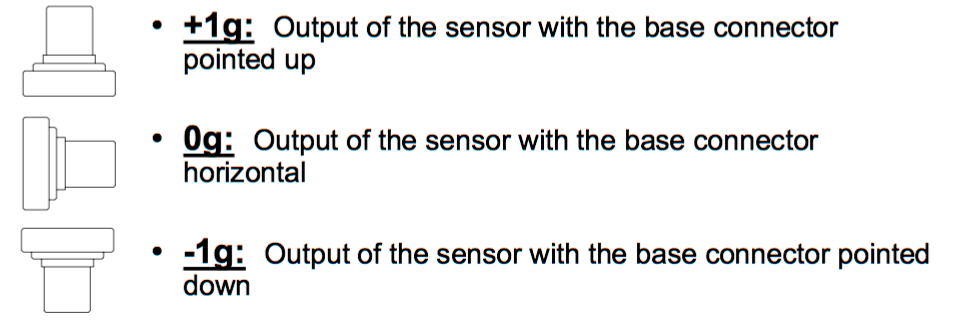
\includegraphics[scale=0.25]{figures/bProblemloesning/g.png}
%	\caption{På figuren ses outputtet i g afhængigt af retning på accelerometeret. \citep{Inspire}}
%	\label{fig:g}
%\end{figure}